% Teselado del tiempo: a qué casillero va cada ciclo, con las ranuras.
% mca_window arma los casilleros dt_* (combinacional, del estado de las
% ranuras) y mca_top los cuenta, junto con la ocupación t_ocup[j].
% El re-armado del disparo (trig_arm_i, del multitrigger) va después de los
% dos casilleros del MCA: t_rearm.
% Fuente: modulos/mca/rtl/mca_window.sv (TIEMPO MUERTO) y mca_top.sv (Relojes).
% Compilar:   pdflatex tm_teselado.tex && pdftocairo -svg tm_teselado.pdf tm_teselado.svg
\documentclass[border=0pt,tikz]{standalone}
\usepackage[utf8]{inputenc}
\usepackage[T1]{fontenc}
\usepackage{lmodern}
\usepackage[none]{hyphenat}
% Estilo común de las figuras TikZ (panoramas y diagramas de bloques).
%
% Cada figura lo incluye con \input{../../figuras/estilo_tikz.tex} (las figuras
% viven en docs/<módulo>/figuras/). Un solo lugar para la paleta, los estilos de
% bloque y el formato de los parámetros: si cambia algo acá, cambia en todas.
%
% La paleta es la misma de docs/figuras/estilo_svg.py y de PALETA en
% modulos/mk/datasheet.py; si se toca un color, se toca en los tres.
%
% Requiere: \usepackage{tikz} (lo da la clase standalone con la opción tikz).

\usetikzlibrary{arrows.meta,positioning,calc,fit,backgrounds,shapes.multipart,
                decorations.markings,shadows}

% ---------------------------------------------------------------- colores ---
\definecolor{azul}{RGB}{108,172,228}      % acondicionamiento
\definecolor{verde}{RGB}{110,214,142}     % captura / histogramas en BRAM
\definecolor{amarillo}{RGB}{252,232,160}  % trigger
\definecolor{naranja}{RGB}{252,206,160}   % camino a DDR
\definecolor{grisr}{RGB}{226,226,226}     % compartido / infraestructura
\definecolor{rojo}{RGB}{240,128,128}      % bus del sistema

% ---------------------------------------------------------------- estilos ---
\tikzset{
  >={Stealth[length=2.4mm,width=1.8mm]},
  % fondo blanco siempre: el SVG se ve igual en modo claro y oscuro
  fondo/.style   = {show background rectangle, inner frame sep=8pt,
                    background rectangle/.style={fill=white, draw=none}},
  bloque/.style  = {draw=black, line width=0.6pt, rounded corners=2pt,
                    align=center, text width=2.2cm, minimum height=1.15cm,
                    inner sep=2pt, font=\scriptsize, fill=#1},
  datos/.style   = {bloque=azul!35},
  trig/.style    = {bloque=amarillo},
  captura/.style = {bloque=verde!55},
  ddr/.style     = {bloque=naranja!70},
  comp/.style    = {bloque=grisr},
  bus/.style     = {bloque=rojo!45},
  % lógica escrita dentro del módulo, sin submódulo propio
  etapa/.style   = {bloque=#1, line width=0.5pt},
  etapa/.default = verde!20,
  % lo que el bitstream no trae (atado a cero, stub, salida muda)
  mudo/.style    = {bloque=white, draw=black!45, dashed, text=black!55},
  %
  % BLOQUE CON PARÁMETROS, en el formato del datasheet: el encabezado lleva el
  % nombre y los parámetros con que lo instancia el padre (NOMBRE=valor, en
  % monoespaciada, uno por línea); el cuerpo, más claro, lo que hace.
  %   \node[datos, param={azul!35}{azul!12}] {\blk{nombre}{} \prm{A=1\\B=2}
  %                                            \nodepart{two} función};
  param/.style 2 args = {rectangle split, rectangle split parts=2,
                         rectangle split part fill={#1, #2}},
  %
  flujo/.style   = {->, line width=0.8pt},
  ctrl/.style    = {->, line width=0.6pt, black!65},
  % la línea que pasa por encima en un cruce: un halo blanco la separa
  cruce/.style   = {preaction={draw=white, line width=3.4pt, -}},
  % marca de ancho de bus: barra oblicua a mitad de la flecha, con el número
  % encima. \draw[flujo, ancho=14] ...; para otra posición, ancho en=0.3.
  ancho/.style   = {decoration={markings, mark=at position \anchopos with {
                      \draw[line width=0.6pt, -] (-0.1,-0.14) -- (0.1,0.14);
                      \node[font=\scriptsize, above=1.5pt] {#1};}},
                    postaction={decorate}},
  % la misma marca en una flecha vertical: el número va a la derecha
  anchov/.style  = {decoration={markings, mark=at position \anchopos with {
                      \draw[line width=0.6pt, -] (-0.14,-0.1) -- (0.14,0.1);
                      \node[font=\scriptsize, right=3pt] {#1};}},
                    postaction={decorate}},
  ancho en/.code = {\def\anchopos{#1}},
  sen/.style     = {font=\scriptsize\ttfamily, inner sep=1.5pt},
  nodo/.style    = {font=\tiny\ttfamily, inner sep=1pt, black!75},
  pin/.style     = {font=\scriptsize, align=center, inner sep=1pt},
  grupo/.style   = {draw=black!55, dashed, line width=0.7pt, rounded corners=4pt},
  canal/.style   = {grupo},
  contenedor/.style = {draw=black!80, line width=1.0pt, rounded corners=6pt},
  % marca numerada: cada número es una fila de la tabla del documento
  marca/.style   = {circle, fill=black, text=white, font=\scriptsize\bfseries,
                    inner sep=0pt, minimum size=4.3mm},
  %
  % DECISIONES (docs/mca/vista_general_mca.md). Cada opción es un bloque, todas
  % entran a un mux (\muxdec, abajo) y el registro que elige entra por abajo.
  % la opción que trae el reset (el comportamiento histórico): borde doble
  defecto/.style = {double=white, double distance=0.8pt, line width=0.45pt},
  % rótulo de la decisión, el mismo Dn del panorama y del documento
  decision/.style = {circle, fill=black, text=white, font=\small\bfseries,
                     inner sep=0pt, minimum size=7mm},
  %
  % LÓGICA (docs/mca/figuras/contabilidad/ y los detalles de las decisiones)
  % registro: caja gris con el triángulo de reloj en el borde de abajo
  registro/.style = {draw=black, line width=0.6pt, fill=grisr, align=center,
                     font=\scriptsize, inner sep=2pt, minimum width=#1,
                     minimum height=0.85cm,
                     path picture={\draw[line width=0.5pt]
                       ([xshift=-1.1mm]path picture bounding box.south) --
                       ([yshift=1.6mm]path picture bounding box.south) --
                       ([xshift=1.1mm]path picture bounding box.south);}},
  registro/.default = 0.8cm,
  % condición de una cadena if / else-if: "sí" sale a la derecha, "no" abajo
  pregunta/.style = {draw=black, line width=0.5pt, rounded corners=7pt,
                     fill=white, font=\scriptsize\ttfamily, align=center,
                     inner sep=2.5pt, minimum height=0.62cm, text width=#1},
  pregunta/.default = 1.9cm,
  si/.style      = {font=\tiny, inner sep=1pt, above, pos=0.12},
  no/.style      = {font=\tiny, inner sep=1pt, left, pos=0.45},
  %
  titulo/.style  = {anchor=north west, font=\small, inner sep=4pt, align=left},
  rotulo/.style  = {anchor=north west, font=\scriptsize\itshape, black!70,
                    inner sep=2pt, align=left},
}

% submódulo: nombre en monoespaciada; lógica propia: nombre en romana
\newcommand{\blk}[2]{{\ttfamily\bfseries #1}\\[1pt]#2}
\newcommand{\etq}[2]{{\bfseries #1}\\[1pt]#2}
\newcommand{\punto}[1]{\fill (#1) circle (1.3pt);}

% Parámetros en el formato del datasheet: NOMBRE=valor en monoespaciada, una
% entrada por celda, hasta cuatro columnas. Una columna: \prm{A=1\\B=2};
% dos: \prm{A=1 & B=2\\C=3}.
\newcommand{\prm}[1]{{\ttfamily\fontsize{5.6}{6.6}\selectfont
  \begin{tabular}{@{}l@{\hspace{7pt}}l@{\hspace{7pt}}l@{\hspace{7pt}}l@{}}#1\end{tabular}}}

\def\anchopos{0.5}

% Mux de una decisión: trapecio con el lado ancho (las entradas) a la izquierda.
% #1 = nombre, #2 = centro, #3 = alto en cm. Deja tres coordenadas:
%   (#1-in)  centro del lado de entradas: las flechas llegan a (#1-in |- opcion.east)
%   (#1-out) la salida
%   (#1-sel) mitad del lado de abajo: por ahí entra el registro que elige
% El rótulo de adentro es opcional: \muxdec{m}{(4,0)}{3.6} y después
% \node[...] at (m) {...}.
\newcommand{\muxdec}[3]{%
  \path #2 coordinate (#1);
  \draw[line width=0.6pt, fill=grisr]
    ($(#1)+(-0.45,{#3/2})$) -- ($(#1)+(0.45,{#3/2-0.35})$) --
    ($(#1)+(0.45,{-#3/2+0.35})$) -- ($(#1)+(-0.45,{-#3/2})$) -- cycle;
  \coordinate (#1-in)  at ($(#1)+(-0.45,0)$);
  \coordinate (#1-out) at ($(#1)+(0.45,0)$);
  \coordinate (#1-sel) at ($(#1)+(0,{-#3/2+0.175})$);}

% El mismo mux rotado 90 grados, para un flujo de arriba hacia abajo: entradas
% por el lado ancho de arriba, salida abajo y el registro que elige por la
% izquierda. #1 = nombre, #2 = centro, #3 = ancho en cm. Deja (#1-in) centro del
% lado de entradas, (#1-out) la salida y (#1-sel) mitad del lado izquierdo.
\newcommand{\muxdecv}[3]{%
  \path #2 coordinate (#1);
  \draw[line width=0.6pt, fill=grisr]
    ($(#1)+({-#3/2},0.45)$) -- ($(#1)+({#3/2},0.45)$) --
    ($(#1)+({#3/2-0.35},-0.45)$) -- ($(#1)+({-#3/2+0.35},-0.45)$) -- cycle;
  \coordinate (#1-in)  at ($(#1)+(0,0.45)$);
  \coordinate (#1-out) at ($(#1)+(0,-0.45)$);
  \coordinate (#1-sel) at ($(#1)+({-#3/2+0.175},0)$);}

% Leyenda de colores + nota. #1 = posición, #2 = color/texto, #3 = nota.
\newcommand{\leyenda}[3]{%
  \begin{scope}[shift={(#1)}, every node/.style={font=\scriptsize}]
    \coordinate (t0) at (-0.5,0);
    \foreach \c/\t [count=\i] in {#2} {
      \pgfmathtruncatemacro\j{\i-1}
      \node[draw, fill=\c, minimum width=4mm, minimum height=3mm, inner sep=0pt,
            right=5mm of t\j.east, anchor=west] (l\i) {};
      \node[right=1.5mm of l\i] (t\i) {\t};
    }
    \node[anchor=north west, black!70, text width=19cm, align=left]
      at (-0.05,-0.3) {#3};
  \end{scope}}

% Lo que dicen los parámetros, para la nota de la leyenda
\newcommand{\notaparam}{\texttt{NOMBRE=valor}: parámetros con que el padre
  instancia el bloque (se omiten los que sólo pasan el del padre sin cambio).}

\tikzset{cuenta/.style = {bloque=grisr, text width=2.5cm, minimum height=0.62cm}}

\begin{document}
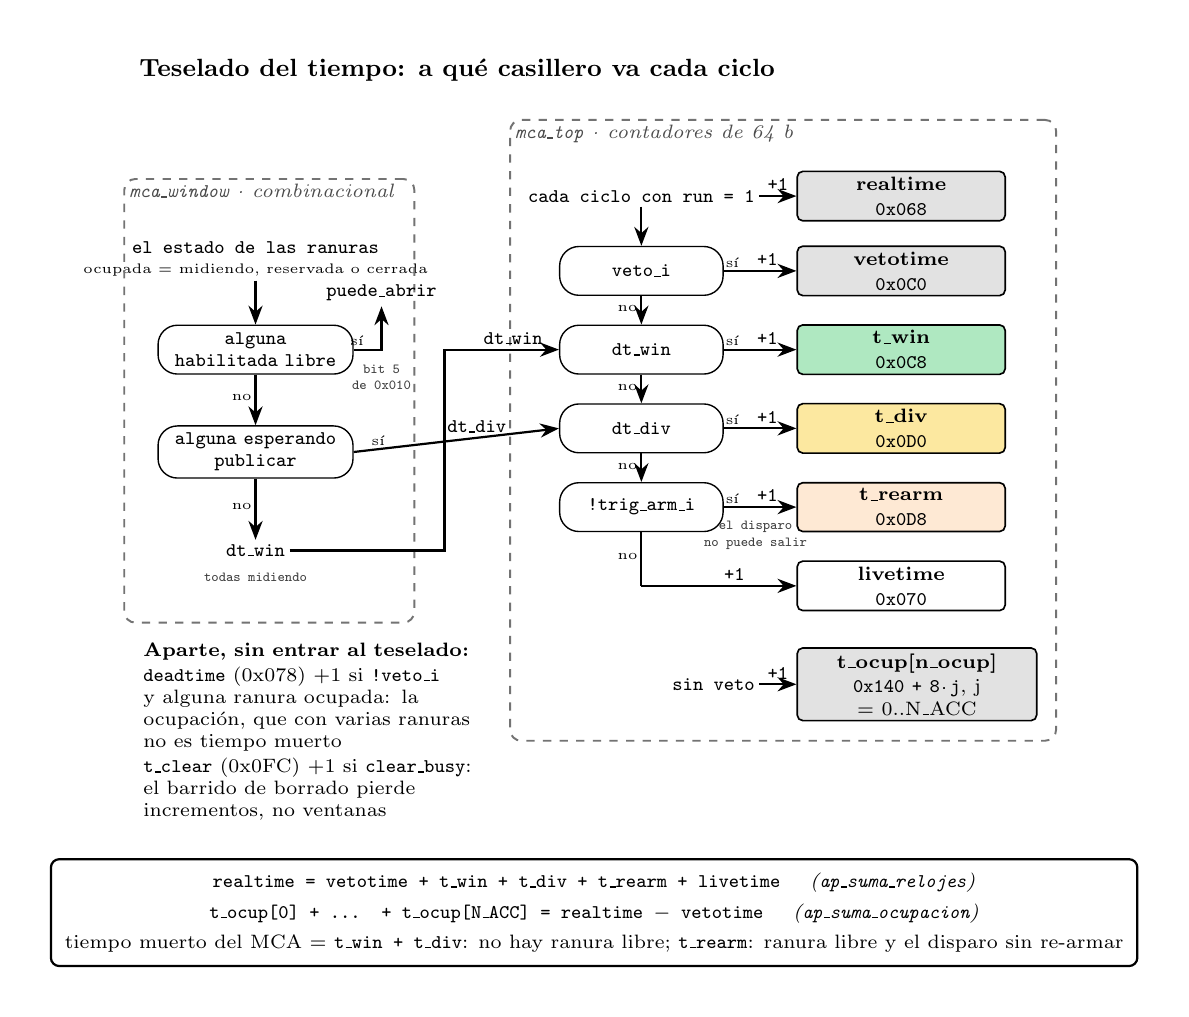
\begin{tikzpicture}[fondo]

\node[anchor=west, font=\small] at (-0.4,3.95)
  {\textbf{Teselado del tiempo: a qué casillero va cada ciclo}};

% ======================================== mca_window: los casilleros dt_* ====
\node[sen, align=center] (ent) at (1.2,1.55) {el estado de las ranuras\\[-1pt]
  \normalfont\tiny ocupada = midiendo, reservada o cerrada};
\node[pregunta=2.3cm] (q1) at (1.2,0.4)  {alguna habilitada libre};
\node[pregunta=2.3cm] (q2) at (1.2,-0.9) {alguna esperando publicar};
\node[sen] (dw) at (1.2,-2.15) {dt\_win};
\draw[flujo] (ent) -- (q1);
\draw[flujo] (q1.south) -- node[no] {no} (q2.north);
\draw[flujo] (q2.south) -- node[no] {no} (dw.north);
\node[nodo, align=left, anchor=north] at (1.2,-2.4) {todas midiendo};
\node[grupo, fit={(-0.35,2.45) (3.1,-2.95)}] (gw) {};
\node[rotulo] at (gw.north west) {\texttt{mca\_window} · combinacional};

% ========================================== mca_top: los relojes de 64 b ====
\node[sen] (run) at (6.1,2.35) {cada ciclo con run = 1};
\node[pregunta] (r0) at (6.1,1.4)  {veto\_i};
\node[pregunta] (r1) at (6.1,0.4)  {dt\_win};
\node[pregunta] (r2) at (6.1,-0.6) {dt\_div};
\node[pregunta] (r3) at (6.1,-1.6) {!trig\_arm\_i};
\coordinate (r4) at (6.1,-2.6);
\draw[flujo] (run) -- (r0);
\foreach \a/\b in {r0/r1, r1/r2, r2/r3}
  \draw[flujo] (\a.south) -- node[no] {no} (\b.north);
\draw[line width=0.8pt] (r3.south) -- node[no] {no} (r4);
\node[nodo, anchor=north, align=center] at (7.55,-1.74) {el disparo\\ no puede salir};

\node[cuenta] (crt) at (9.4,2.35) {\etq{realtime}{\texttt{0x068}}};
\node[cuenta] (c0)  at (9.4,1.4)  {\etq{vetotime}{\texttt{0x0C0}}};
\node[cuenta, fill=verde!55]  (c1) at (9.4,0.4)  {\etq{t\_win}{\texttt{0x0C8}}};
\node[cuenta, fill=amarillo]  (c2) at (9.4,-0.6) {\etq{t\_div}{\texttt{0x0D0}}};
\node[cuenta, fill=naranja!45] (c3) at (9.4,-1.6) {\etq{t\_rearm}{\texttt{0x0D8}}};
\node[cuenta, fill=white]     (c4) at (9.4,-2.6) {\etq{livetime}{\texttt{0x070}}};
\draw[flujo] (run) -- node[sen, above] {+1} (crt);
\foreach \k in {0,1,2,3}
  \draw[flujo] (r\k.east) -- node[si] {sí} node[sen, above, pos=0.6] {+1} (c\k.west);
\draw[flujo] (r4) -- node[sen, above, pos=0.6] {+1} (c4.west);

% la ocupacion, en paralelo
\node[cuenta, text width=2.9cm] (oc) at (9.6,-3.85)
  {\etq{t\_ocup[n\_ocup]}{\texttt{0x140 + 8·j}, j = 0..N\_ACC}};
\node[sen, anchor=east] (no) at (7.6,-3.85) {sin veto};
\draw[flujo] (no) -- node[sen, above] {+1} (oc.west);
\node[grupo, fit={(4.55,3.2) (11.25,-4.45)}] (gt) {};
\node[rotulo] at (gt.north west) {\texttt{mca\_top} · contadores de 64 b};

% ================================== los casilleros cruzan de un lado al otro
\draw[flujo] (q1.east) -- node[si] {sí} (2.8,0.4) -- (2.8,0.95) node[sen, above] {puede\_abrir};
\draw[flujo] (q2.east) -- node[si] {sí} node[sen, above, pos=0.6] {dt\_div} (r2.west);
\draw[flujo] (dw.east) -- (3.6,-2.15) |- node[sen, above, pos=0.8] {dt\_win} (r1.west);
\node[nodo, anchor=north, align=center] at (2.8,0.25) {bit 5\\ de 0x010};

% ============================================== lo que no entra al teselado
\node[anchor=north west, font=\scriptsize, align=left, text width=4.6cm]
  at (-0.35,-3.2)
  {\textbf{Aparte, sin entrar al teselado:}\\[1pt]
   \texttt{deadtime} (0x078) $+$1 si \texttt{!veto\_i} y alguna ranura ocupada: la
   ocupación, que con varias ranuras no es tiempo muerto\\[1pt]
   \texttt{t\_clear} (0x0FC) $+$1 si \texttt{clear\_busy}: el barrido de borrado
   pierde incrementos, no ventanas};

% ================================================================ invariantes
\node[draw=black, line width=0.8pt, rounded corners=3pt, fill=white, inner sep=5pt,
      align=center, font=\scriptsize] at (5.5,-6.75)
  {\texttt{realtime = vetotime + t\_win + t\_div + t\_rearm + livetime}
   \quad {\itshape(\texttt{ap\_suma\_relojes})}\\[3pt]
   \texttt{t\_ocup[0] + … + t\_ocup[N\_ACC] = realtime $-$ vetotime}
   \quad {\itshape(\texttt{ap\_suma\_ocupacion})}\\[3pt]
   tiempo muerto del MCA $=$ \texttt{t\_win + t\_div}: no hay ranura libre;
   \texttt{t\_rearm}: ranura libre y el disparo sin re-armar};

\end{tikzpicture}
\end{document}
